\subsubsection*{exemple d'exécution du \textit{swap}}

\begin{itemize}
\item \textbf{étape 0}

\begin{center}
\begin{tikzpicture}[scale=0.5]
%%%%%%%%%%%%%%%%%%%%%%%%%%%%%%%%%%%%%%%%%%%%%%%%%%%%%%%%
% STYLE
\tikzstyle{case}=[rectangle,draw,minimum width=0.5cm,minimum height=0.5cm, font=\tiny]
\tikzstyle{op}=[circle,draw]
\tikzstyle{txt}=[font=\tiny]

\tikzset{link/.style={->,>=stealth'}}

%%%%%%%%%%%%%%%%%%%%%%%%%%%%%%%%%%%%%%%%%%%%%%%%%%%%%%%%
% NODES
\node[case] (T00) at (0, 0) {$4$};
\node[case] (T01) at (1, 0) {$8$};
\node[case] (T02) at (2, 0) {$11$};
\node[case] (T03) at (3, 0) {$16$};

\node[case] (T06) at (6, 0) {$2$};
\node[case] (T07) at (7, 0) {$7$};
\node[case] (T08) at (8, 0) {$19$};
\node[case] (T09) at (9, 0) {$18$};

\node[case] (T12) at (12, 0) {$0$};
\node[case] (T13) at (13, 0) {$15$};
\node[case] (T14) at (14, 0) {$3$};
\node[case] (T15) at (15, 0) {$17$};
\node[case] (T16) at (16, 0) {$16$};

\node[txt] (txt0) at (3,1) {$indice = 3$};
\node[txt] (txt1) at (8,1) {$indice = 2$};
\node[txt] (txt2) at (15,1) {$indice = 3$};

\node[txt] (txt3) at (1.5,-1) {proc\_deb};
\node[txt] (txt4) at (14,-1) {proc\_fin};

\node[txt,align=left] (txt5) at (-3,0) {
$proc\_deb=0$\\
$proc\_fin=2$
};
%%%%%%%%%%%%%%%%%%%%%%%%%%%%%%%%%%%%%%%%%%%%%%%%%%%%%%%%
% LINKS
\draw[link] (txt0) -> (T03);
\draw[link] (txt1) -> (T08);
\draw[link] (txt2) -> (T15);
\end{tikzpicture}
\end{center}

\item \textbf{étape 1}

Les indices proc\_deb et proc\_fin sont valides, on échange et on modifie les indices.\\

\begin{center}
\begin{tikzpicture}[scale=0.5]
%%%%%%%%%%%%%%%%%%%%%%%%%%%%%%%%%%%%%%%%%%%%%%%%%%%%%%%%
% STYLE
\tikzstyle{case}=[rectangle,draw,minimum width=0.5cm,minimum height=0.5cm, font=\tiny]
\tikzstyle{op}=[circle,draw]
\tikzstyle{txt}=[font=\tiny]

\tikzset{link/.style={->,>=stealth'}}

%%%%%%%%%%%%%%%%%%%%%%%%%%%%%%%%%%%%%%%%%%%%%%%%%%%%%%%%
% NODES
\node[case] (T00) at (0, 0) {$4$};
\node[case] (T01) at (1, 0) {$8$};
\node[case] (T02) at (2, 0) {$11$};
\node[case] (T03) at (3, 0) {$3$};

\node[case] (T06) at (6, 0) {$2$};
\node[case] (T07) at (7, 0) {$7$};
\node[case] (T08) at (8, 0) {$19$};
\node[case] (T09) at (9, 0) {$18$};

\node[case] (T12) at (12, 0) {$0$};
\node[case] (T13) at (13, 0) {$15$};
\node[case] (T14) at (14, 0) {$16$};
\node[case] (T15) at (15, 0) {$17$};
\node[case] (T16) at (16, 0) {$16$};

\node[txt] (txt0) at (4,1) {$indice = 4$};
\node[txt] (txt1) at (8,1) {$indice = 2$};
\node[txt] (txt2) at (14,1) {$indice = 2$};

\node[txt] (txt3) at (1.5,-1) {proc\_deb};
\node[txt] (txt4) at (14,-1) {proc\_fin};

\node[txt,align=left] (txt5) at (-3,0) {
$proc\_deb=0$\\
$proc\_fin=2$
};
%%%%%%%%%%%%%%%%%%%%%%%%%%%%%%%%%%%%%%%%%%%%%%%%%%%%%%%%
% LINKS
\draw[link] (txt0) -> (4, 0.5);
\draw[link] (txt1) -> (T08);
\draw[link] (txt2) -> (T14);
\end{tikzpicture}
\end{center}

\item \textbf{étape 2}

L'indice de proc\_deb n'est pas bon, on incrémente proc\_deb et on recommence.

\begin{center}
\begin{tikzpicture}[scale=0.5]
%%%%%%%%%%%%%%%%%%%%%%%%%%%%%%%%%%%%%%%%%%%%%%%%%%%%%%%%
% STYLE
\tikzstyle{case}=[rectangle,draw,minimum width=0.5cm,minimum height=0.5cm, font=\tiny]
\tikzstyle{op}=[circle,draw]
\tikzstyle{txt}=[font=\tiny]

\tikzset{link/.style={->,>=stealth'}}

%%%%%%%%%%%%%%%%%%%%%%%%%%%%%%%%%%%%%%%%%%%%%%%%%%%%%%%%
% NODES
\node[case] (T00) at (0, 0) {$4$};
\node[case] (T01) at (1, 0) {$8$};
\node[case] (T02) at (2, 0) {$11$};
\node[case] (T03) at (3, 0) {$3$};

\node[case] (T06) at (6, 0) {$2$};
\node[case] (T07) at (7, 0) {$7$};
\node[case] (T08) at (8, 0) {$19$};
\node[case] (T09) at (9, 0) {$18$};

\node[case] (T12) at (12, 0) {$0$};
\node[case] (T13) at (13, 0) {$15$};
\node[case] (T14) at (14, 0) {$16$};
\node[case] (T15) at (15, 0) {$17$};
\node[case] (T16) at (16, 0) {$16$};

\node[txt] (txt1) at (8,1) {$indice = 2$};
\node[txt] (txt2) at (14,1) {$indice = 2$};

\node[txt] (txt3) at (7.5,-1) {proc\_deb};
\node[txt] (txt4) at (14,-1) {proc\_fin};

\node[txt,align=left] (txt5) at (-3,0) {
$proc\_deb=1$\\
$proc\_fin=2$
};
%%%%%%%%%%%%%%%%%%%%%%%%%%%%%%%%%%%%%%%%%%%%%%%%%%%%%%%%
% LINKS
\draw[link] (txt1) -> (T08);
\draw[link] (txt2) -> (T14);
\end{tikzpicture}
\end{center}

\item \textbf{étape 3}

Les indices sont bons, on échange et on modifie les indices.

\begin{center}
\begin{tikzpicture}[scale=0.5]
%%%%%%%%%%%%%%%%%%%%%%%%%%%%%%%%%%%%%%%%%%%%%%%%%%%%%%%%
% STYLE
\tikzstyle{case}=[rectangle,draw,minimum width=0.5cm,minimum height=0.5cm, font=\tiny]
\tikzstyle{op}=[circle,draw]
\tikzstyle{txt}=[font=\tiny]

\tikzset{link/.style={->,>=stealth'}}

%%%%%%%%%%%%%%%%%%%%%%%%%%%%%%%%%%%%%%%%%%%%%%%%%%%%%%%%
% NODES
\node[case] (T00) at (0, 0) {$4$};
\node[case] (T01) at (1, 0) {$8$};
\node[case] (T02) at (2, 0) {$11$};
\node[case] (T03) at (3, 0) {$3$};

\node[case] (T06) at (6, 0) {$2$};
\node[case] (T07) at (7, 0) {$7$};
\node[case] (T08) at (8, 0) {$15$};
\node[case] (T09) at (9, 0) {$18$};

\node[case] (T12) at (12, 0) {$0$};
\node[case] (T13) at (13, 0) {$19$};
\node[case] (T14) at (14, 0) {$16$};
\node[case] (T15) at (15, 0) {$17$};
\node[case] (T16) at (16, 0) {$16$};

\node[txt] (txt1) at (9,1) {$indice = 3$};
\node[txt] (txt2) at (13,1) {$indice = 1$};

\node[txt] (txt3) at (7.5,-1) {proc\_deb};
\node[txt] (txt4) at (14,-1) {proc\_fin};

\node[txt,align=left] (txt5) at (-3,0) {
$proc\_deb=1$\\
$proc\_fin=2$
};
%%%%%%%%%%%%%%%%%%%%%%%%%%%%%%%%%%%%%%%%%%%%%%%%%%%%%%%%
% LINKS
\draw[link] (txt1) -> (T09);
\draw[link] (txt2) -> (T13);
\end{tikzpicture}
\end{center}

\item \textbf{étape 4}

Les indices sont bons, on échange et on modifie les indices.

\begin{center}
\begin{tikzpicture}[scale=0.5]
%%%%%%%%%%%%%%%%%%%%%%%%%%%%%%%%%%%%%%%%%%%%%%%%%%%%%%%%
% STYLE
\tikzstyle{case}=[rectangle,draw,minimum width=0.5cm,minimum height=0.5cm, font=\tiny]
\tikzstyle{op}=[circle,draw]
\tikzstyle{txt}=[font=\tiny]

\tikzset{link/.style={->,>=stealth'}}

%%%%%%%%%%%%%%%%%%%%%%%%%%%%%%%%%%%%%%%%%%%%%%%%%%%%%%%%
% NODES
\node[case] (T00) at (0, 0) {$4$};
\node[case] (T01) at (1, 0) {$8$};
\node[case] (T02) at (2, 0) {$11$};
\node[case] (T03) at (3, 0) {$3$};

\node[case] (T06) at (6, 0) {$2$};
\node[case] (T07) at (7, 0) {$7$};
\node[case] (T08) at (8, 0) {$15$};
\node[case] (T09) at (9, 0) {$0$};

\node[case] (T12) at (12, 0) {$18$};
\node[case] (T13) at (13, 0) {$19$};
\node[case] (T14) at (14, 0) {$16$};
\node[case] (T15) at (15, 0) {$17$};
\node[case] (T16) at (16, 0) {$16$};

\node[txt] (txt1) at (10,1) {$indice = 4$};
\node[txt] (txt2) at (12,1.5) {$indice = 0$};

\node[txt] (txt3) at (7.5,-1) {proc\_deb};
\node[txt] (txt4) at (14,-1) {proc\_fin};

\node[txt,align=left] (txt5) at (-3,0) {
$proc\_deb=1$\\
$proc\_fin=2$
};
%%%%%%%%%%%%%%%%%%%%%%%%%%%%%%%%%%%%%%%%%%%%%%%%%%%%%%%%
% LINKS
\draw[link] (txt1) -> (10, 0.5);
\draw[link] (txt2) -> (T12);
\end{tikzpicture}
\end{center}

\item \textbf{étape 5}

L'indice de proc\_deb est faux, on incrémente proc\_deb.

\begin{center}
\begin{tikzpicture}[scale=0.5]
%%%%%%%%%%%%%%%%%%%%%%%%%%%%%%%%%%%%%%%%%%%%%%%%%%%%%%%%
% STYLE
\tikzstyle{case}=[rectangle,draw,minimum width=0.5cm,minimum height=0.5cm, font=\tiny]
\tikzstyle{op}=[circle,draw]
\tikzstyle{txt}=[font=\tiny]

\tikzset{link/.style={->,>=stealth'}}

%%%%%%%%%%%%%%%%%%%%%%%%%%%%%%%%%%%%%%%%%%%%%%%%%%%%%%%%
% NODES
\node[case] (T00) at (0, 0) {$4$};
\node[case] (T01) at (1, 0) {$8$};
\node[case] (T02) at (2, 0) {$11$};
\node[case] (T03) at (3, 0) {$3$};

\node[case] (T06) at (6, 0) {$2$};
\node[case] (T07) at (7, 0) {$7$};
\node[case] (T08) at (8, 0) {$15$};
\node[case] (T09) at (9, 0) {$0$};

\node[case] (T12) at (12, 0) {$18$};
\node[case] (T13) at (13, 0) {$19$};
\node[case] (T14) at (14, 0) {$16$};
\node[case] (T15) at (15, 0) {$17$};
\node[case] (T16) at (16, 0) {$16$};

\node[txt] (txt2) at (12,1) {$indice = 0$};

\node[txt] (txt3) at (14,-1) {proc\_deb et proc\_fin};

\node[txt,align=left] (txt5) at (-3,0) {
$proc\_deb=2$\\
$proc\_fin=2$
};
%%%%%%%%%%%%%%%%%%%%%%%%%%%%%%%%%%%%%%%%%%%%%%%%%%%%%%%%
% LINKS
\draw[link] (txt2) -> (T12);
\end{tikzpicture}
\end{center}

\item \textbf{étape 6}

On s'arrête et on broadcast l'indice de proc\_deb qui est $0$ ajouté à l'indice de début du block. La séparation pour les appels récursifs est donc la suivante :

\begin{center}
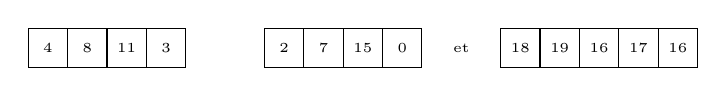
\begin{tikzpicture}[scale=0.5]
%%%%%%%%%%%%%%%%%%%%%%%%%%%%%%%%%%%%%%%%%%%%%%%%%%%%%%%%
% STYLE
\tikzstyle{case}=[rectangle,draw,minimum width=0.5cm,minimum height=0.5cm, font=\tiny]
\tikzstyle{op}=[circle,draw]
\tikzstyle{txt}=[font=\tiny]

\tikzset{link/.style={->,>=stealth'}}

%%%%%%%%%%%%%%%%%%%%%%%%%%%%%%%%%%%%%%%%%%%%%%%%%%%%%%%%
% NODES
\node[case] (T00) at (0, 0) {$4$};
\node[case] (T01) at (1, 0) {$8$};
\node[case] (T02) at (2, 0) {$11$};
\node[case] (T03) at (3, 0) {$3$};

\node[case] (T06) at (6, 0) {$2$};
\node[case] (T07) at (7, 0) {$7$};
\node[case] (T08) at (8, 0) {$15$};
\node[case] (T09) at (9, 0) {$0$};

\node[case] (T12) at (12, 0) {$18$};
\node[case] (T13) at (13, 0) {$19$};
\node[case] (T14) at (14, 0) {$16$};
\node[case] (T15) at (15, 0) {$17$};
\node[case] (T16) at (16, 0) {$16$};

\node[txt] (txt2) at (10.5,0) {et};
%%%%%%%%%%%%%%%%%%%%%%%%%%%%%%%%%%%%%%%%%%%%%%%%%%%%%%%%
% LINKS
\end{tikzpicture}
\end{center}

\end{itemize}